\section{Modelado, Control y Algoritmos de Navegación}



\subsection{Bloque de Cinemática y Control de Tracción}


\subsubsection{Modelo dinámico e Identificación de la Planta del Motor GA12-N20}
Desde el punto de vista físico, el motor DC (GA12-N20) no responde de forma instantánea a los cambios de tensión debido a la inercia del rotor y la fricción de los engranajes. A su vez, existe una relación proporcional entre el ciclo de trabajo de la señal PWM aplicada a través del puente H y la velocidad angular alcanzada en estado permanente.

Para representar este comportamiento dinámico en el dominio de Laplace, la planta se modela como un sistema de primer orden:

\[G(s) = \frac{\Omega(s)}{U(s)} = \frac{K}{\tau s + 1}\]

Donde
\begin{itemize}
	\item {$\Omega(s)$} es la velocidad angular de salida de la rueda, expresada en $[rad/s]$.
	\item {$U(s)$} es la señal de control aplicada al puente H, expresada en unidades de PWM (Duty Cycle $[0-100\%]$)
	\item {$K$} es la ganancia del sistema, expresada en $[(rad/s)/unidad PWM]$.
	\item {$\tau$} es la constante de tiempo mecánica, expresada en milisegundos $[ms]$, que representa el tiempo necesario para que la respuesta alcance el $63,2\%$ de su valor de estado permanente.
\end{itemize}

Para obtener los valores de $K$ y $\tau$ para cada rueda (izquierda y derecha) se aplica un escalón de tensión partiendo del reposo y se registra la velocidad angular en función del tiempo mediante el sensor magnético AS5600.

\paragraph{Identificación de la Ganancia $K$}
Una vez alcanzado el régimen permanente, se calcula $K$ como el cociente entre la velocidad angular alcanzada y el ciclo de trabajo definido por el escalón en U(s).

\paragraph{Identificación de la constante de tiempo $\tau$}
Se determina identificando el instante de tiempo donde $t=\tau$ tal que la velocidad angular alcanzada sea del $63,2\%$.



\subsubsection{Lazo Interno: Diseño y Sintonización de Controlador PI del Motor GA12-N20}

\paragraph{Diseño en el Dominio Continuo}~\\
Habiendo identificado la función de transferencia de la planta (motor), es posible ahora plantear un lazo cerrado por PID de la velocidad angular de un motor, y por lo tanto de la rueda correspondiente.


\begin{figure}[H]
	\centering
	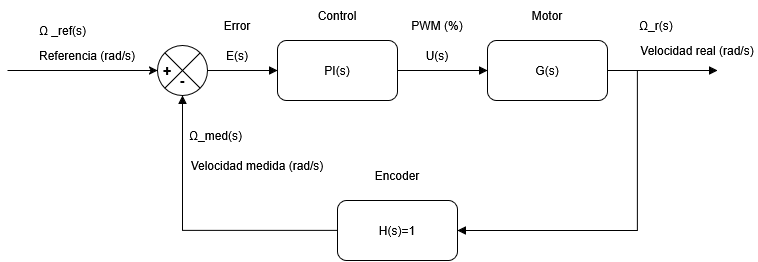
\includegraphics[width=0.8\textwidth]{Imagenes/Lazo Interno-Motor.png}
	\caption{Lazo interno de control de un motor. (MEJORAR, CAMBIAR PI POR C(S))}
	\label{fig:lazointernomotor}
\end{figure}

Donde:
\begin{itemize}
	\item {$\Omega\_$ref(s)} es la velocidad angular de referencia para el motor.
	\item {$E(s)$} es el error entre la velocidad de referencia y la velocidad medida.
	\item {$C(s)$} es el control proporcional e integral.
	\item {$U(s)$} es la señal PWM enviada al motor por $C(s)$.
	\item {$G(s)$} es la función de transferencia del motor.
	\item {$\Omega\_$r(s)} es la velocidad angular real que tiene el motor.
	\item {$H(s)=1$} es la función de transferencia del encoder, se la asume sin retrasos.
	\item {$\Omega\_$med(s)} es la velocidad medida por el encoder, utilizada para el cálculo del error.
\end{itemize}

Siendo que la función de transferencia de la planta es

\[G(s) = \frac{K}{\tau s + 1}\]

Es posible plantear un control por PI

\[C(s) = K_p + K_i/s = K_p(\frac{s+K_i/K_p}{s})\]

Donde la función de transferencia a lazo abierto es (renombrando $\tau$ como $\tau_{la}$, constante de tiempo de lazo abierto)

\[LA(s) = C(s)G(s) =  K_p(\frac{s+K_i/K_p}{s}) \frac{K}{\tau_{la} s + 1}\]

Analizando la función de lazo abierto, vemos es que posible cancelar uno de sus polos, eligiendo $K_i$ y $K_p$ tal que

\[\frac{K_i}{K_p} = \frac{1}{\tau_{la}} => K_i=\frac{K_p}{\tau_{la}}\]

Queda entonces la función de transferencia a lazo abierto

\[LA(s) = \frac{K_pK}{s\tau_{la}}\]

Al cerrar el lazo, la función de transferencia a lazo cerrado queda

\[LC(s) = \frac{LA(s)}{1+LA(s)H(s)} = \frac{\frac{K_pK}{s\tau_{la}}}{1+\frac{K_pK}{s\tau_{la}}1}\] 
\[LC(s) = \frac{1}{\frac{1}{K_pK}s+1} = \frac{1}{\tau_{lc}s+1}\]

Donde $\tau_{;c}$ es la constante de tiempo a lazo cerrado. Siendo que depende del valor de la constante $K_p$, nos da un grado de libertad para definir el tiempo de respuesta que queremos que tenga el lazo cerrado de control.

\[\tau(K_p) = \frac{1}{K_pK}\]
\[K_i(K_p) = \frac{K_p}{\tau}\]


\paragraph{Criterio del Muestreo}~\\
En el mundo real, es imposible integrar cada instante de tiempo. El intervalo de muestreo del estado del lazo cerrado (medición del sensor y computo de la lógica en consecuencia) se deberá de hacer cada cierto $\Delta t$. Para garantizar que el controlador digital represente fielmente el comportamiento diseñado en el dominio continuo, el intervalo de muestreo $\Delta t$ debe ser lo suficientemente chico respecto a la velocidad de respuesta del lazo cerrado ($\tau_{lc}$).

Un período de muestreo del orden de la constante de tiempo ($\Delta t\approx\tau_{lc}$) resulta inaceptable por: Dado que $t=\tau_{lc}$ la velocidad angular ya ha alcanzado el $63,2\%$ de su estado permanente para cuando se hace el primer muestreo. Esto impide detectar las variaciones bruscas de velocidad a lo largo del recorrido hacia el regimen permanente. Por otro lado, la aproximación de la integral por suma de rectángulos $e[k]\Delta t$ asume que el error varía suavemente entre muestras. Un $\Delta t$ elevado induce error por discretización sustancial.

Por lo tanto, se toma el criterio empírico de diseño, el cual establece que se deben tomar al menos entre 5 y 10 muestras durante la constante de lazo cerrado:

\[\Delta t <= \frac{\tau_{lc}}{10}\]

Dado que la constante de tiempo del motor a lazo cerrado es de $\tau_{lc}\approx LLENAR$, se toma entonces un valor de $\Delta t = LLENAR$.

\paragraph{Discretización}~\\
Para trasladar el lazo de control diseñado en el dominio continuo $s$ al microcontrolador, se requiere discretizar la ecuación diferencial en el dominio del tiempo t:

\[u(t)=K_pe(t)+K_i\int_{0}^{t} e(m) \,dm\]

Evaluando $t = k\Delta t$ (donde $k$ representa el número de muestra actual y $\Delta t$ el período de muestreo elegido anteriormente), se obtiene la ecuación en diferencias:

\[u[k]=K_pe[k]+\sum_{i=1}^{k} e[i]\Delta t\]

Donde la integral se aproxima mediante una suma de Riemann (rectángulos de ancho $\Delta t$ y altura $e[k]$).

El cálculo directo de la sumatoria $\sum_{i=1}^{k} e[i]\Delta t$ requeriría de almacenar todo el historial de errores en memoria RAM, lo que incrementaría el tiempo de procesamiento a medida que el robot opera.

Para resolver esto, es posible expresar la integral k-ésima de manera recursiva, en función del cálculo anterior. Siendo $I[k]$ el término integral:

\[I[k] = I[k-1] + e[k]\Delta t\]

De esta forma el algoritmo solo conserva en memoria un único valor, resultando en la ecuación en diferencias final:

\[u[k]=K_pe[k]+K_iI[k]\]

VER DE HACER EL CODIGO ACA O EN ALGUN LADO, TAMBIEN MENCIONAR QUE EN EL CODIGO SE DEBERIA LIMITAR LA SALIDA DEL CONTROLADOR PI (u(s)) A MAX 100\% y MIN 0\%.

\subsubsection{Cinemática Directa: Odometría Primaria a partir de Encoders}


\subsubsection{Lazo Externo: Control Cinemático Polar para Seguimiento Punto a Punto}


\subsubsection{Cinemática Inversa}




\subsection{Bloque de Mapeo y Estimación de Posición}


\subsubsection{Análisis Experimental de Deriva Odométrica en theta}


\subsubsection{Corrección de orientación mediante IMU}


\subsubsection{Modelado del sensor TOF y construcción de la grilla de ocupación}




\subsection{Bloque de Navegación Autónoma}


\subsubsection{Estrategia de exploración y selección de metas}


\subsubsection{Algoritmo de evasión de obstáculos}




\subsection{Integración de Lazos y Arquitectura de Control Global}


\subsubsection{Diagrame unificado del sistema de control}


\subsubsection{Máquina de estados y lógica de selección de modos}